\section{Data characteristics}
\label{sec:data_charcteristics}

Data characteristics, distribution and error visualization of 6 datasets:

Table data characteristics

Diagrams of \#nnz (sort by nnz), distinct items. 
% TODO add references
\begin{table}[!t]
\caption{\label{tab:dataset_sizes}Datasets}
\centering
\begin{tabular}{r|K|K|K|K|H|K}
\toprule
 & \colCenter{\#rows} & \colCenter{\#cols} & \colCenter{Clean}  & \colCenter{Dirty}  & \colCenter{\#Cat} & \colCenterNoRight{\#Numeric}\\
\midrule
beers                & 2410     & 11     &    233 \textsc{KB}              & 255 \textsc{KB}                    & 8                    & 3                    \\
flights              & 2376     & 7      &    173 \textsc{KB}              & 155 \textsc{KB}                    & 7                    & 0                    \\
hospital             & 1000     & 20     &    303 \textsc{KB}              & 303 \textsc{KB}                     & 20                   & 0                     \\
movies               & 7390     & 17     &    4400 \textsc{KB}              & 4600 \textsc{KB}                    & 14                   & 3                    \\
rayyan               & 1000     & 11     &    273 \textsc{KB}              & 273 \textsc{KB}                    & 9                    & 2                     \\
tax                  & 200000   & 15     &    14,6 \textsc{MB}             & 14,6 \textsc{MB}                   & 10                   & 5                    \\
\bottomrule    
\end{tabular}
\end{table}

\subsection{Datasets}
To real-world datasets are used. In Table~\ref{tab:dataset_sizes} datasets and their sizes are presented.
% TODO variance in rows to column ratios
% TODO string vs numeric vs categorical 
% Why dirty is bigger?

\subsection{Data characteristics}
The main goal is to maintain the characteristics of the dirty data while generating larger datasets. 
% TODO Why mean
% TODO Why variance is not preserved
% TODO Why distincts 
% TODO Data statistics plot/ table

\begin{figure}[!t]
    \centering 
    \centering
\begin{subfigure}{0.4\textwidth}
    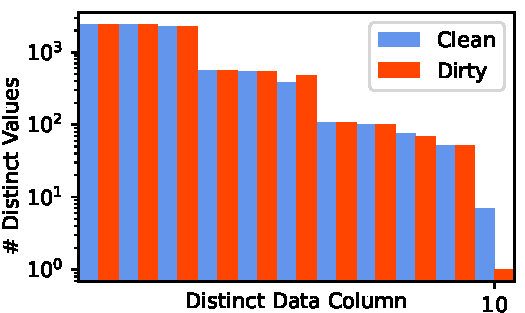
\includegraphics[width=\textwidth]{figures/plot/distinct/beers_distinct/combined.pdf}
    \caption{\label{exp:d1}Bears}
    \label{exp:distincts_bears}
\end{subfigure}
\hfill
\begin{subfigure}{0.4\textwidth}
    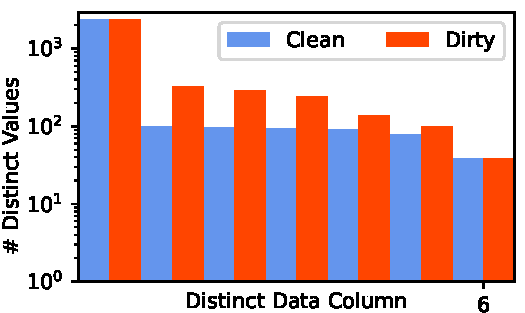
\includegraphics[width=\textwidth]{figures/plot/distinct/flights_distinct/combined.pdf}
    \caption{Flights}
    \label{exp:distincts_flights}
\end{subfigure}
\hfill
\begin{subfigure}{0.4\textwidth}
    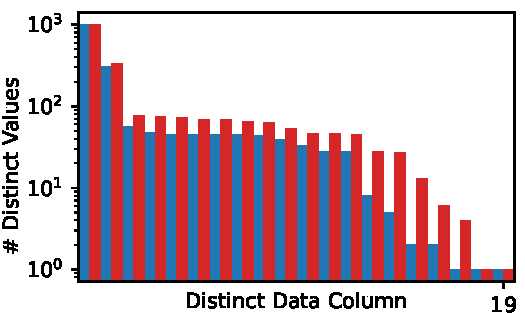
\includegraphics[width=\textwidth]{figures/plot/distinct/hospital_distinct/combined.pdf}
    \caption{Hospital}
    \label{fig:distincts_hospitals}
\end{subfigure}
\hfill
\begin{subfigure}{0.4\textwidth}
    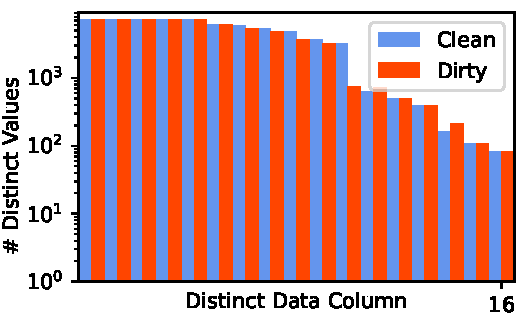
\includegraphics[width=\textwidth]{figures/plot/distinct/movies_distinct/combined.pdf}
    \caption{Movies}
    \label{exp:distincts_movies}
\end{subfigure}
\hfill
\begin{subfigure}{0.4\textwidth}
    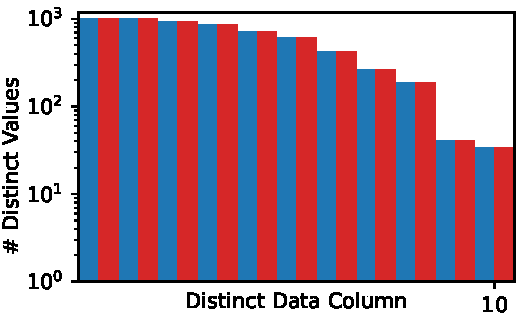
\includegraphics[width=\textwidth]{figures/plot/distinct/rayyan_distinct/combined.pdf}
    \caption{Rayyan}
    \label{exp:distincts_rayyan}
\end{subfigure}
\hfill
\begin{subfigure}{0.4\textwidth}
    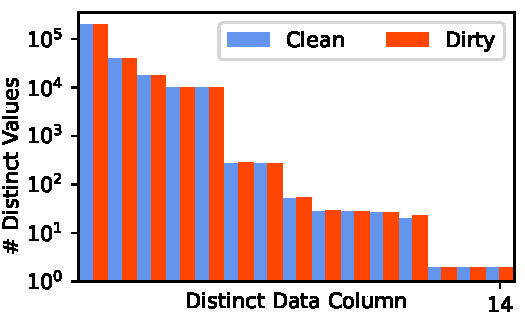
\includegraphics[width=\textwidth]{figures/plot/distinct/tax_distinct/combined.pdf}
    \caption{Tax}
    \label{exp:distincts_tax}
\end{subfigure}
\hfill
% TODO describe 
        
\caption{Distinct values distribution of clean and dirty datasets}
\label{exp:distinct_values_datasets}
\end{figure}
Figure \ref{exp:distinct_values_datasets} shows the number of distinct values and their frequencies in each dataset. 

\subsection{Error distribution}
To preserve the error distribution in generated dataset, error characteristics of the original dirty are %TODO.
\begin{table}[!t]
\caption{\label{tab:dirty_num_errors}Dirty dataset error characteristics}
\begin{tabular}{r|l|l|l|l|l}
\toprule
                     & Outliers & Typos & Missing values & Replacement & Swaps \\ \midrule
beers                & 0        & 254   & 4170           & 0                & 0       \\
flights              & 0        & 2243  & 0              & 0                & 314     \\
hospital             & 0        & 417   & 92             & 0                & 0       \\
movies               & 0        & 982   & 6346           & 141              & 0       \\
rayyan               & 0        & 649   & 75             & 224              & 0       \\
tax                  & 2        & 1367  & 588            & 1200             & 4       \\ \bottomrule
\end{tabular}
\end{table}
% TODO Replacement vs Flipped category vs Flipped value
In Table \ref{tab:dirty_num_errors} number of errors in every dataset.

% TODO Each column which type of error is present in which column.
\begin{figure}[!t]
    \centering 
    \centering
\begin{subfigure}{0.4\textwidth}
    \includegraphics[width=\textwidth]{example-image-a}
    \caption{\label{exp:d1}Bears}
    \label{exp:barplot_error_count_bears}
\end{subfigure}
\hfill
\begin{subfigure}{0.4\textwidth}
    \includegraphics[width=\textwidth]{example-image-a}
    \caption{Flights}
    \label{exp:barplot_error_count_flights}
\end{subfigure}
\hfill
\begin{subfigure}{0.4\textwidth}
    \includegraphics[width=\textwidth]{example-image-a}
    \caption{Hospital}
    \label{fig:barplot_error_count_hospital}
\end{subfigure}
\hfill
\begin{subfigure}{0.4\textwidth}
    \includegraphics[width=\textwidth]{example-image-a}
    \caption{Movies}
    \label{exp:barplot_error_count_movies}
\end{subfigure}
\hfill
\begin{subfigure}{0.4\textwidth}
    \includegraphics[width=\textwidth]{example-image-a}
    \caption{Rayyan}
    \label{exp:barplot_error_count_rayyan}
\end{subfigure}
\hfill
\begin{subfigure}{0.4\textwidth}
    \includegraphics[width=\textwidth]{example-image-a}
    \caption{Tax}
    \label{exp:distincts_tax}
\end{subfigure}
\hfill
\begin{subfigure}{0.4\textwidth}
    \includegraphics[width=\textwidth]{example-image-a}
    \caption{Toy}
    \label{exp:barplot_error_count_toy}
\end{subfigure}
\caption{Number of errors in each dataset}
\label{exp:barplot_error_counts_datasets}
\end{figure}